\documentclass[a4paper, 11pt]{report}
\usepackage[margin=2.25cm]{geometry}
\usepackage{url}
\usepackage[utf8]{inputenc}
\usepackage{graphicx}
\usepackage{lipsum} 
\usepackage{titlesec}
\usepackage[T1]{fontenc}
\usepackage{enumerate}
\usepackage[shortlabels]{enumitem}
\usepackage{hyperref}
\usepackage{xurl}
\usepackage{listings}
\usepackage{color}
\usepackage[table]{xcolor}
\usepackage{svg}
\usepackage{float}
\usepackage{subcaption}
\usepackage{tikz}
\usepackage{amsmath}
\usepackage{amsfonts}
\usepackage{stmaryrd}
\usepackage{amssymb}
\usepackage{bbm}
\usepackage[style=ieee]{biblatex}

\usetikzlibrary{automata, positioning, arrows}
\tikzset{->, >=stealth, node distance=4cm, every state/.style={thick, fill=gray!10},
initial text=$ $,
}

\addbibresource{DocIMT.bib}

\hypersetup{
    colorlinks=true,
    citecolor=black,
    linkcolor=black,
    urlcolor= blue
}

\DeclareCaptionFormat{custom}
{
    \textsc{#1#2}#3
}

\DeclareCaptionLabelSeparator{custom}{ -- }

\captionsetup{    
    format=custom,
    labelsep=custom
}

\renewcommand{\thesection}{\Roman{section}}

\titleformat{\section}{\LARGE\bfseries}{\thesection. \ }{0pt}{}
\titleformat{\subsection}{\Large\bfseries}{}{0pt}{}
\titleformat{\subsection}{\large\bfseries}{}{0pt}{}

\lstdefinestyle{default}{
    basicstyle=\normalfont\ttfamily,
	frame=shadowbox,
	backgroundcolor=\color{white},
}

\lstset{style=default}

\begin{document}

    \begin{titlepage}
    
        \begin{center}
        
            \vspace*{1cm}
            
            \huge
            \textsc{\textbf{4G Analysis Program Documentation}}
            
            \LARGE
            
            \vspace*{1cm}
            
            Killian CALLAC
            
            \Large
            
            \vspace*{1cm}
            
            IMT Atlantique Rennes
            
            \vspace*{1cm}
            
            July 2022
            
            \vspace*{1cm}
            
            Internship supervised by Xavier LAGRANGE, \\
            professor at IMT Atlantique, \\
            and Julien SAINT-MARTIN, research engineer.
            
            
            \vspace*{1.5cm}
            
            
\includegraphics[width=0.5\textwidth]{IMT_Atlantique_logo_RVB_Baseline_400x272.jpg}
            
            
        \end{center}
    
    \end{titlepage}
    
    \setcounter{tocdepth}{3}
    \tableofcontents
    
    \newpage
    
    \addcontentsline{toc}{section}{Acknowledgments}
    \section*{Acknowlegements}
    I want to thank first Mr. Xavier LAGRANGE and Mr. Julien SAINT-MARTIN for the help they gave me during the realization of this project, and for their trust. \newline
    
    I want also thank the SRCD department team of IMT Atlantique for their warm and human welcome. \newline
    
    Finally, I would also like to thank Mr. Mathieu GOESSENS, teacher at the University of Rennes 1, and Mr. Erwan ABGRALL, specialist in cybersecurity, who helped me when I was searching my internship.
    
    \newpage
    
    
    \addcontentsline{toc}{section}{Introduction}
    \section*{Introduction}
    At IMT Atlantique, the Adopnet team uses since 2019 a 4G network analysis software. This software, written with the Python programming language, has for main purpose to visualize on a map measurements taken on the 4G LTE mobile network. Usually, these measurements are done in exterior, with one or several devices connected to a measurement tool. Originally, this tool was the ZK-Samp tool, consisting in a measurement device which was taking measurements from one or several phones connected to it. The tool was taking global signal measurements, geolocated and associated to a timestamp. The original program has been developed in order to allow the user to visualize easily global signal measurements in a more concise way, to easily link these measurements to a particular network cell \cite{trieu_visualization_2019}. \newline
    
    However, the ZK-Samp tool of the Adopnet team doesn't work anymore, and the company which was producing it no longer exists. The Adopnet team uses now Accuver Xcal-M, a software which can do geolocated global measurements over the network like the ZK-Samp tool, but can also do measurements for each detected cells as well, no matter if the user equipment is actively connected to these cells. Xcal-M produces a data format (Accuver Open Format, or AOF) which is slightly different of the data format produced by the ZK-Samp tool, and it is necessary to adapt the original analysis program to this new format. The format of some intermediate files needs also to be changed for readability reasons, and the visualization must also be improved due to the fact the file format of Xcal-M is more rich.\newline
    
    The purpose of our work on this program is to implement previously mentioned changes ; this report aims to document these changes, for usability, understanding and maintainability purposes. We will first focus on a presentation of the software and how use it, before we present data processings methods used in the software, to present next the visualization part of the program.

    \newpage
    
    \section{Global presentation of the software}
    
    In this part, we will first remind the overall structure of a 4G cellular network, the perimeter of the software and the related concepts. We will then present the program itself from an user perspective, by detailing its main functions.
    
    \subsection{Remind of 4G network concepts and perimeter of the software}
    Cellular networks are composed of three main parts: the user terminal, commonly called User Equipement (UE) ; an access network (commonly called RAN, for Radio Access Network), which allows the User Equipement to communicate by radio access to a core network ; and the core network, which manage numerous inner functions of the network, as the registering of users, the billing policy, call controls and the connection to exteriors networks (e.g. Internet network) \cite{bouguen_lte_2012}. \newline
    
    4G networks are based on the Long Term Evolution (LTE) norm, which uses as access network the Evolved Universal Terrestrial Radio Access Network (e-UTRAN), and as core network the Evolved Packet Core (EPC) \cite{bouguen_lte_2012}. \newline
    
    The program has as perimeter the User Equipment and the e-UTRAN network: the User Equipment is used here to do measurements, and these measurements are done on the e-UTRAN network. \newline
    
    \begin{figure}[H]
    \centering
    \includesvg[width=0.8\textwidth]{lte_arch.drawio.svg}
    \caption{LTE network architecture}
    \label{LTE Network Architecture}
    \end{figure}
    
    A Radio Access Network uses base stations to communicate with User Equipments. These base stations are equipped of several antennas, with can send data to and receive data from User Equipments \cite{bouguen_lte_2012}. Every base station covers a geographical zone called a cell. Antennas of base stations  are oriented to cover a specific zone of the cell, called a sector. Usually, cells are divided in three sectors, every sectors often covering an angle of approximately 120° around the base station ; however, it is possible to encounter cells with more or less sectors. \newline
    
    In the e-UTRAN network, bases stations are called eNodeB. \newline
    
    \begin{figure}[H]
    \centering
    \includesvg[width=0.5\textwidth]{cells.drawio.svg}
    \caption{e-UTRAN cells spatial organization. Each hexagonal cell is covered by an eNodeB ; in case of trisectorization, cells are divided in three parts, delimited by green lines on the figure.}
    \label{e-UTRAN Cells}
    \end{figure}
    
    eNodeB can emits data on several frequency bands. These frequency bands are designated by a code called EARFCN (Extended Absolute Radio Frequency Channel Number). Data sent from the UE to the network (Uplink, or UL) and data sent from the network to the UE (Downlink, or DL), use different frequency bands. \newline
    
    We will present more detailed aspects of the LTE network in next parts.
    
    \subsection{Software functionalities}
    
    The tool is usable through a graphical user interface which allows the user to access main functionalities. Textual traces can also be found on a command line interface.
    
    \subsubsection{Initial data processing functionalities}
    
    \begin{figure}[H]
    \centering
    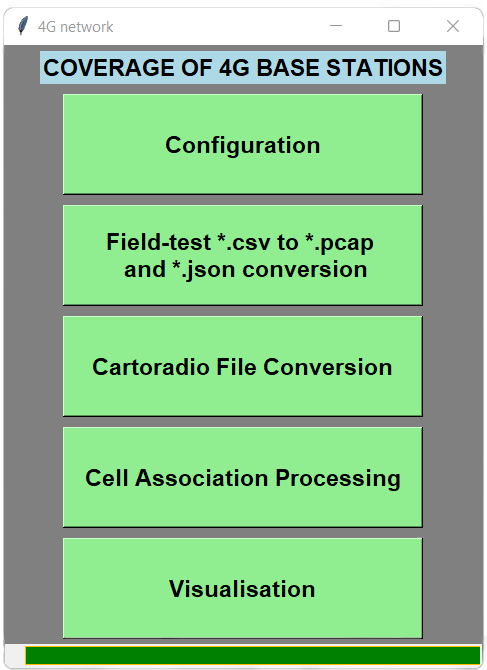
\includegraphics[width=0.5\textwidth]{fenetre.png}
    \caption{Software user interface.}
    \label{Software user interface}
    \end{figure}
    
    The user must first click on the "Configuration" button and choose in a dialog a directory: in this directory will be produced output files from the program. \newline
    
    Next, the user can use other functionalities of the program. The \textbf{Field-test *.csv to *.pcap and AOF-like *.csv conversion} button allow the user to choose an Accuver Open Format measurement file, and produce a PCAP trace readable by Wireshark, and a CSV\footnote{Commas Separated Values, textual format readable by spreadsheets which represents data tabularly.} file constructed like an AOF file, which contains information about cells, geolocations of measurement points, and measurements classed by EARFCN and cell identifiers. Every measurement in this output file possess a timestamp, which locates information in time. \newline
    
    The user can also use the button \textbf{Cartoradio File Conversion} to produce information about antennas in several AOF-shaped CSV output files, from datasets from the ANFR\footnote{Agence Nationale des Fréquences, french organization that manages the allocation of frequency bands of the country.} website Cartoradio. Exportable datasets from Cartoradio contains several CSV files. Two of them are used  here: the \texttt{Sites\_Cartoradio.csv} and \texttt{Antennes\_Emetteurs\_Bandes\_Cartoradio.csv}: the first file contains information about base stations, their geolocation, their height and several information about the place were they are located, and the second file contains data about each antenna found on the exported zone, such as directivity information (azimuth), used technology (LTE for 4G), frequency bands or operators. Two output files are produced per operator, a "sites" (eg. \texttt{sites\_SFR.csv}) file which associates each antenna to its base station data and to a sector delimitation. Sector delimitation data are also produced separately in the file for the visualization. "Rejected" files (eg. \texttt{rejected\_SFR.csv} contain same kind of information, except antennas contained in this file are below the ground level: separate these antennas from others allow the software to not visualize underground base station, which can be encountered for example in metro tunnels and stations, in order to avoid to overestimate the cell range, which is in reality very limited. \newline
    
    \begin{figure}[H]
    \centering
    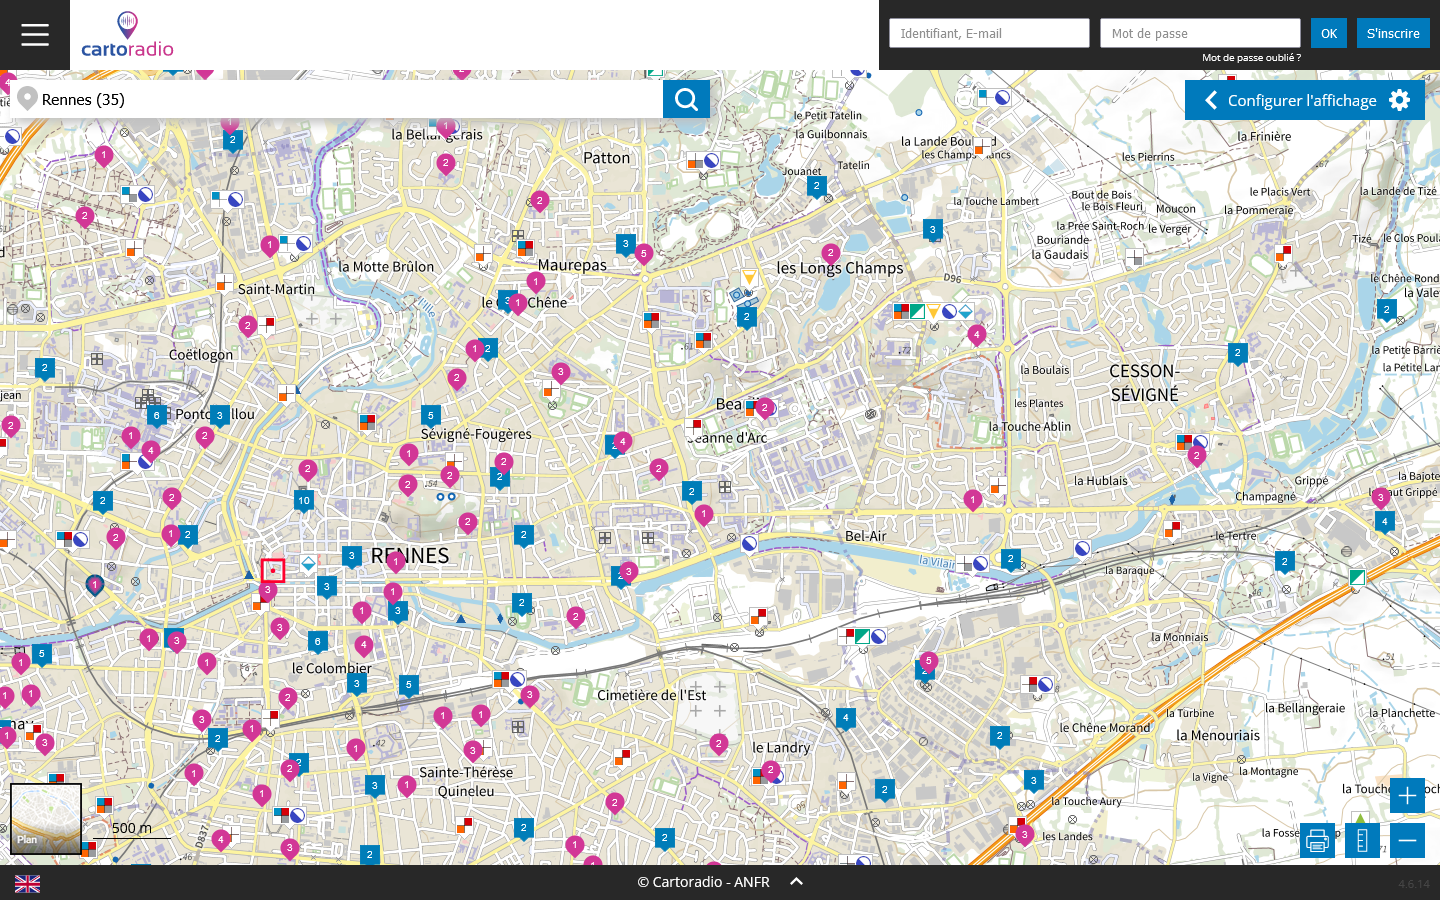
\includegraphics[width=0.8\textwidth]{Cartoradio_UI.png}
    \caption{Cartoradio user interface.}
    \label{Cartoradio user interface}
    \end{figure}
    
    The \textbf{Cell Association Processing} feature take as input a "sites" file produced by the Cartoradio File Conversion step and a CSV file produced by the Field-test functionality. This feature associates antennas from the first file with measurement points from the second file: details of the association calculation will be given in the next parts. Groups of points, corresponding to a given cell and a given EARFCN, are also created. Measurement points associated with antennas and measurement values, measurement values and sectors data used by the visualization are stored in a final output CSV file.
    
    \subsubsection{Data visualization}
    The software allows the user to visualize measurements points on a graphical interface. This interface is in fact a local web app which can be used through a web browser. \newline
    
    \begin{figure}[H]
    \centering
    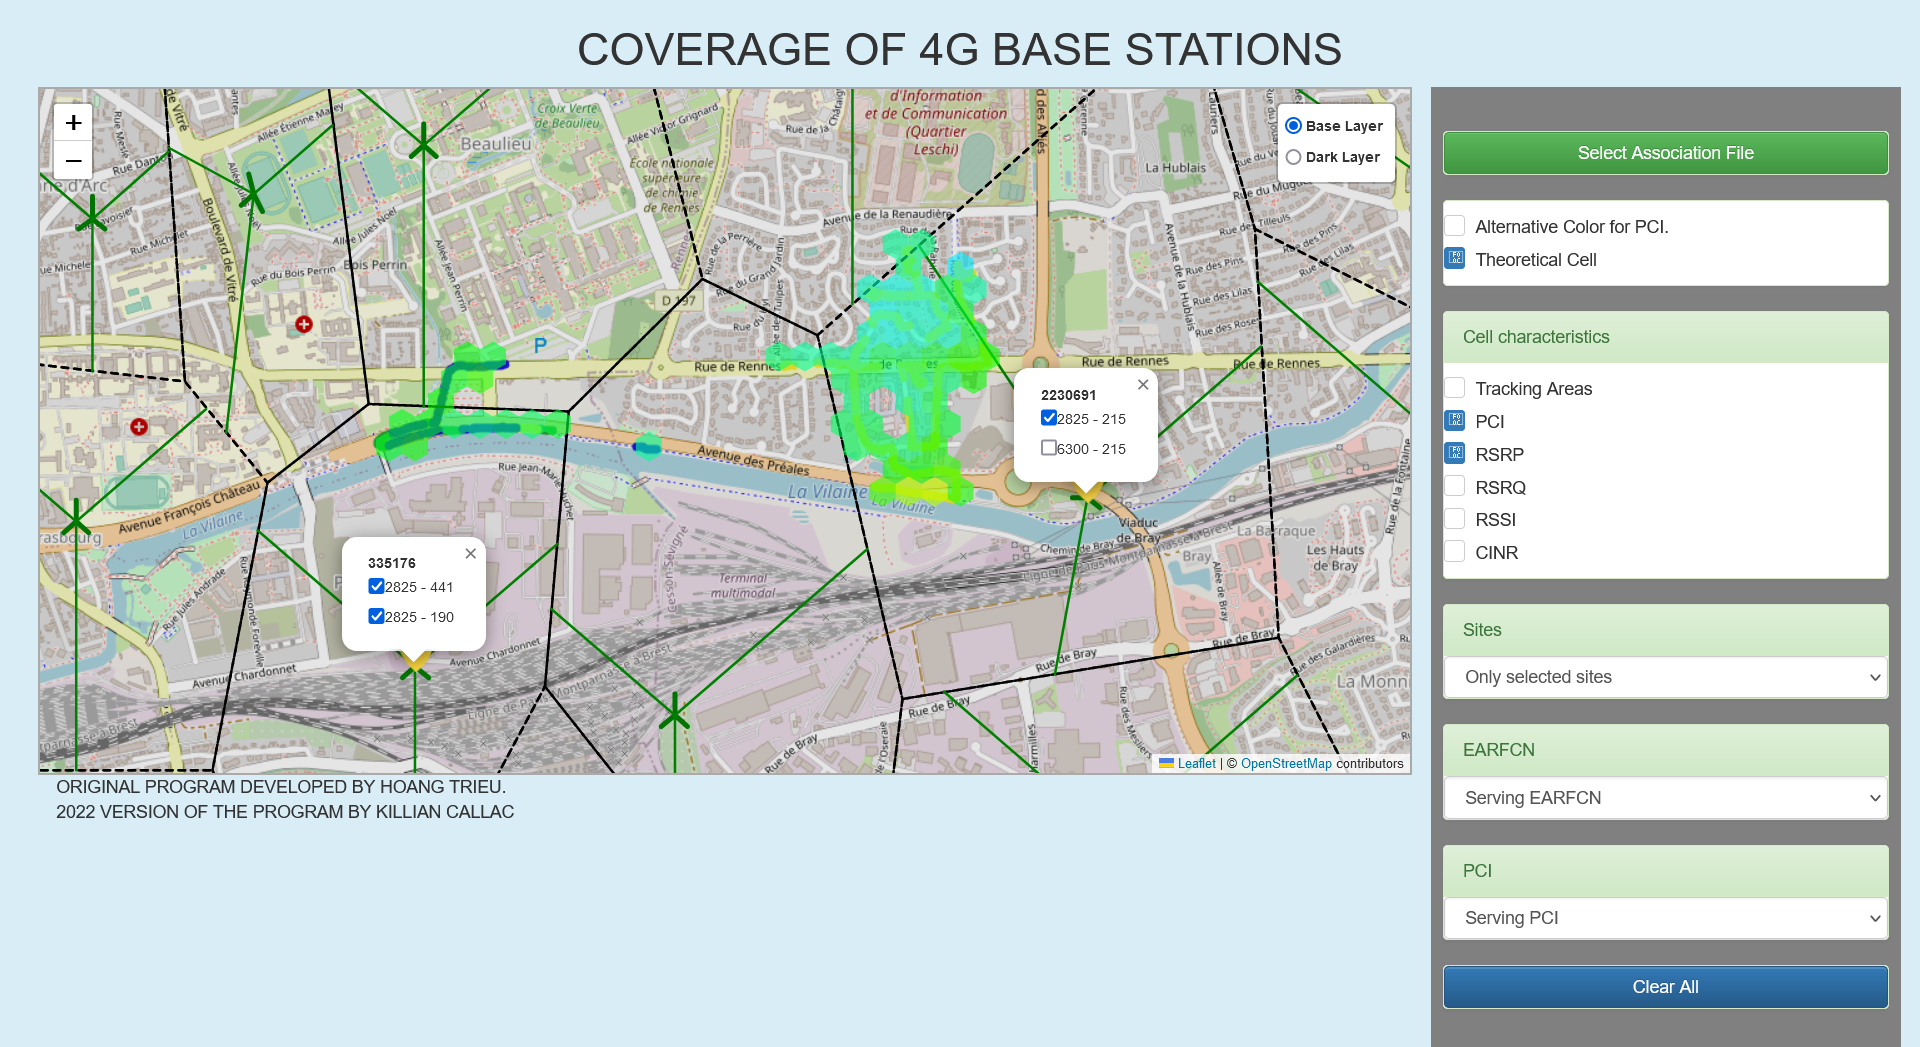
\includegraphics[width=0.9\textwidth]{web_UI.png}
    \caption{Measurement visualization interface.}
    \label{Measurement visualization interface}
    \end{figure}
    
    The web interface includes a map, which is used to display measurement, and several lateral panels, used to set visualization preferences. The user can load an association CSV file and can display data contained in the file with the "Select Association File" button. This action will have as an effect to display green "crosses", which corresponds to loaded base station: branchs of these "crosses" indicate in fact the directivity of each antennas of base stations. Base stations with a yellow mark on them are base stations associated to measurement points; numbers of these associated base stations can be seen by clicking on yellow marks. \newline
    
    The user can use the "Theoretical Cells" checkbox at the left of the screen to show the Voronoi diagram which estimates the delimitation of the cells. From each base station, several thin green lines that extends from the base station to the limits of the cell can be seen: these lines indicate the limits of sectors associated with antennas. \newline
    
    Still at the left of the screen, a group called "Measurements" can be seen. This groups contains several checkboxes. The first checkbox, "Tracking Area", displays colored measurement points on the map. Each color corresponds to an unique Tracking Area. The "PCI" checkbox displays these points, but with each color corresponding to a Physical Cell Identifier, which identify uniquely each cell. An alternative color choice can be displayed by checking "Alternative Color for PCI". Checkboxes RSRP, RSSI, RSRQ and CINR displays different signal measurements around geolocated points, using an hexagonal colored tiling to represent the intensity of these measurement. The meaning of RSRP, RSRQ, RSSI and CINR will be explained later. \newline
    
    In the "Sites" menu, it is possible to select two options: "All sites" display all measurements from all sites, "Only selected sites" allows the user to chose which ERAFCN / PCI from an associated it wants to see, by clicking on the associated site pins and check the corresponding EARFCN / PCI. \newline
    
    In the bottom right corner of the screen, frames "EARFCN" and "PCI" contains two drop-down lists, which respectively allow the user to choose an EARFCN and a PCI. If an EARFCN and / or PCI is chosen, measurements will be filtered on the map, allowing to only see global measurements with corresponding EARFCN / PCI. Other possible choices are serving EARFCNs and PCIs, which displays EARFCNs and / or PCIs from the serving antennas, and "All EARFCNs" / "All PCIs" options allows the user to visualise global measurements for all EARFCNs and PCIs. \newline
    
    \subsection{Python program structure}
    
    The Python program is divided into several modules, several of them being entirely dedicated to one of the  functionalities of the software. \newline
    
    The bootable part of the program is situated in the module \texttt{Interface.py}, which contains the \texttt{GUI} class, which is the main Frame (window) of the program. The library used for the interface is \texttt{tkinter}, which is distributed in Python standard library. This module must be run in order to execute the program. \newline
    
    The module \texttt{xcalyzer.py} is dedicated to the "Field-test *.csv to *.pcap and AOF-like *.csv conversion" functionality. It contains the parsing class \texttt{XcalConverter} for the AOF format, which arranges data stored in the input AOF file to produce the output file of this functionality. \newline
    
    The module \texttt{cartoradio.py} contains functions to read Cartoradio "sites" and "antennas" files, and produce output files containing information about antennas for each operator. \newline
    
    The module \texttt{association.py} contains the class \texttt{CellAssociator}, which is used to associate antennas data and measurements. \newline
    
    There is also several utility modules: \texttt{csvtools.py}, which contains class to read custom AOF-like CSV format, which will be described later, \texttt{dictutils.py}, which is a module that contains utility functions to manage data dictionaries, and \texttt{pcaputils.py}, used to generate easily data in PCAP files. Legacy module \texttt{constantPath.py} is also used as it provides useful paths functions. \newline
    
    Several libraries are also used in the program. These libraries are the following:
    
    \begin{itemize}
        \item Pandas: used to do data treatments (grouping, natural joins, filtering) on massive datasets.
        \item SciPy: used here to calculate theoretical cells.
        \item Shapely: used to do geometrical calculations.
        \item Numpy: used here to do vectorized calculations.
    \end{itemize}
    
    \begin{figure}[H]
    \centering
    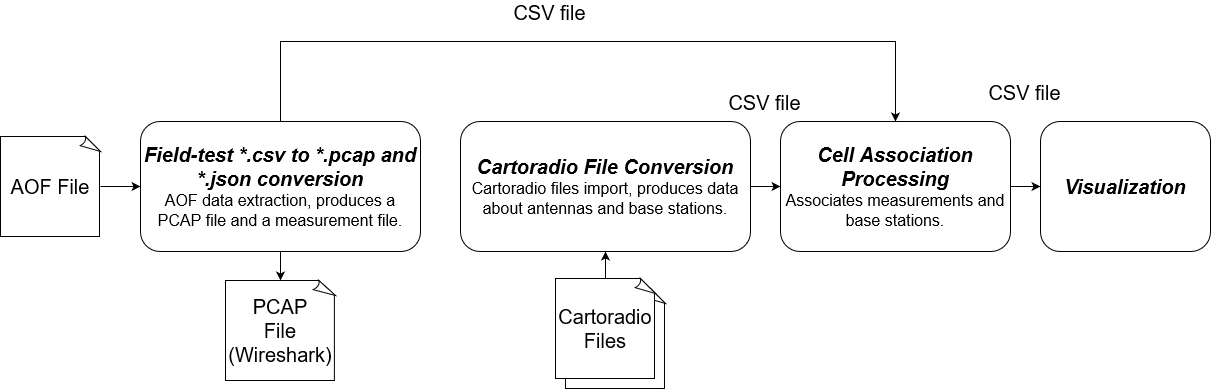
\includegraphics[width=0.9\textwidth]{boites.png}
    \caption{Software architecture.}
    \label{Software architecture.}
\end{figure}
    
    \newpage
    
    \section{Software data formats and processings}
    In this section, we will present data formats used as inputs and outputs of the software, and related data processings. We will first present the Accuver Open Format (AOF), used as main input format, then we will define the common format used in each functionality of the software, before we present data treatments on these formats.
    
    \subsection{Accuver Open Format presentation}
    Accuver Xcal uses as output format the "Accuver Open Format" (AOF), a textual format which contains measurement traces following a textual, tabular structure. This format is in fact an extension of the Comma Separated Values (CSV) format, commonly supported by most of spreadsheets softwares. Basically, the CSV format arranges data tabularly, each line of the file corresponding to a row. Columns are separated by a separator character (usually the \texttt{','} character, but others characters can be used in other languages, e.g. \texttt{';'} in French). The AOF format uses as separator character \texttt{'|'}. Each row, and so each line, corresponds to a data trace, with fields separated by the separator character. \newline
    
    The most notable particularity of the AOF format is the fact the file is splitted in three parts, delimited by two delimiters which take each one line. The first part, the \texttt{AOF\_Information} part (delimited by \texttt{<AOF\_Information Start>} and \texttt{<AOF\_Information End>}, contains data about Accuver Xcal, such as the version number. The second part, the \texttt{Description} part (delimited by \texttt{<Description Start>} and \texttt{Description End>}), defines each trace type, and its fields names and types. A trace definition is divided in two lines, each line beginning by the trace name: the first line defines the name of each field, and the second line defines types of these fields. The third part, the \texttt{Content} part (delimited by \texttt{<Content Start>} and \texttt{<Content End>}), contains data itself, with each trace identified by its name, at the beginning of the line. \newline
    
    A great advantage of the AOF format is, because it is based on the CSV format, it can be read on a spreadsheet software. A filter can be used to visualize each trace type, with corresponding headers and data types visible at the top of the table.
    
    \begin{figure}[H]
    \centering
    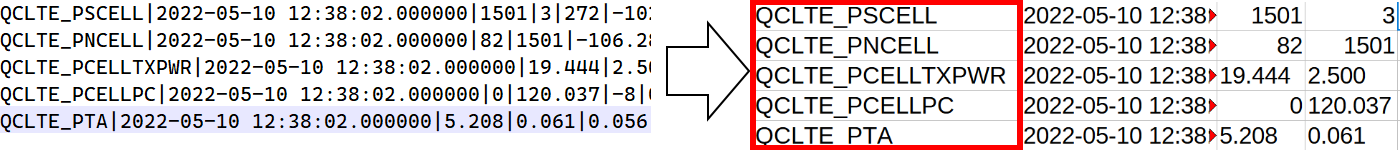
\includegraphics[width=0.80\textwidth]{aof.png}
    \caption{AOF file, visualized on a text editor and on a spreadsheet. Figure by Killian CALLAC, extracted from \cite{callac_rapport_2022}}.
    \label{AOF and CSV}
    \end{figure}
    
    \subsection{"Customized AOF" CSV output format definition}
    
    Each data processing step of the software produces different output files. These files use a specific data format. We based this format on the AOF file format, to replace JSON\footnote{JavaScript Object Notation} output files previously used, which were not easily readable by a human. As we previously mentioned it, the AOF file format is more easier to read, especially when displayed by a spreadsheet, a quality which is appreciated for an output file format. \newline
    
    \subsubsection{Syntax of the file format}
    Formally, the syntax of the format is, using Python regular expressions\footnote{\url{https://docs.python.org/3/library/re.html\#regular-expression-syntax}}:

\begin{figure}[H]
    \centering
    \begin{lstlisting}[showspaces=true]
DEFINE\n
(\w+\|\w+(\|\w+)*\n)*
CONTENT\n
(\w+\|([^\s|]| )*(\|([^\s|]| )*)*\n)*\end{lstlisting}
    \caption{Syntax of the AOF / CSV file format.}
    \label{Syntax of the AOF / CSV file format}
\end{figure}
    
    The file is divided in two parts, a \texttt{DEFINE} part and a \texttt{CONTENT} part. In the \texttt{DEFINE} part, data entry types are specified: at the beginning of the line, a non-empty string, using only alphanumeric characters, defines the name of the entry. Following fields names, separated by the character \texttt{'|'}, should be defined with a non-empty, alphanumeric string; each entry definition, which take one line, should contain at least an entry name and one field name. There can be zero, one ore more entry definitions. The \texttt{CONTENT} part contains data entries, which occupy one line each. Data entries are identified by entries names (non-empty alphanumeric strings), and several values, which can be empty, and made of all characters which are not spacing characters, unless the \texttt{'|'} character, which is used to separate values of an entry. \newline
    
    More informally, an example of valid CSV / AOF file can be found below:
    
    \begin{figure}[H]
        \centering
        \begin{lstlisting}[numbers=left, numberstyle=\ttfamily]
DEFINE
entryName1|fieldName1|fieldName2|fieldName3
entryName2|fieldName4|fieldName5|fieldName6|fieldName7|fieldName8
entryName3|fieldName9|fieldName10
CONTENT
entryName1|10|test|50
entryName2|never|gonna|give|you|up
entryName1|something|test|
entryName3|3.14|42
entryName3||
entryName1||1|10|
entryName2|never|gonna|let|you|down\end{lstlisting}
        \caption{Example of a valid AOF/CSV text. Note there is no need to have same length entries, or non empty values in entries.}
        \label{fig:my_label}
    \end{figure}
    
    In the program, this file format is handled by the module \texttt{csvtools}. This module contains a writer class, \texttt{CSVWriter}, and a reader class, \texttt{CSVReader}. \texttt{CSVWriter} requires to write in the file an header, which is a dictionary used to define the \texttt{DEFINE} part, which use as keys names of entries and as values lists of field names . A line can be added to the \texttt{CONTENT} file with a list beginning with the corresponding entry name, followed by values, associated by indexes to corresponding fields in the header. \newline
    
    \texttt{CSVReader} reads file data. The file is firstly opened temporarily, the corresponding header is generated first following the \texttt{DEFINE} part, and syntactic and semantic controls are done on the file. Secondly, the file is closed and reopened, and the user can read line per line the \texttt{CONTENT} section. \newline
    
    As the language of the file does not define nested structures, and follows a linear sequence, we can identify it as a regular language, which can be recognized by a finite state machine. This finite state machine use as symbols first elements of each lines: at each transition, a new line is read. For the first reading of the file, we implemented the following finite state machine, using actions (numbered in \textbf{bold} on transitions) to do syntactic and semantic controls:
    
    \begin{figure}[H]
        \centering
        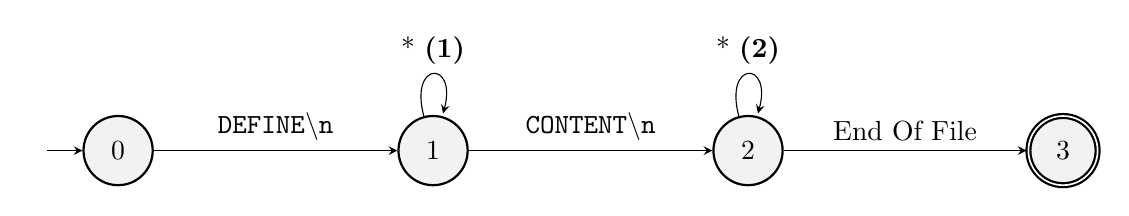
\begin{tikzpicture}
            \node[state, initial](s0) {0};
            \node[state, right of=s0](s1) {1};
            \node[state, right of=s1](s2) {2};
            \node[state, accepting, right of=s2](s3) {3};
            
            \draw (s0) edge[above] node{\texttt{DEFINE\textbackslash n}} (s1)
                  (s1) edge[loop above] node{* \textbf{(1)}} (s1)
                  (s1) edge[above] node{\texttt{CONTENT\textbackslash n}} (s2)
                  (s2) edge[loop above] node{* \textbf{(2)}} (s2)
                  (s2) edge[above] node{End Of File} (s3);
        \end{tikzpicture}
        \caption{AOF-like CSV recognition finite state machine. "*" symbols mean here every possible symbol can be accepted; note that a valid symbol on the FSM can be refused by the action associated to the transition.}
        \label{AOF-like CSV recognition finite state machine}
    \end{figure}
    
    Corresponding actions are:
    
    \begin{enumerate}[label=\textbf{(\arabic*)}: ]
        \item Use the first symbol of the line as entry name. Verify that the line contains field names. Verify that the entry name follows the pattern \texttt{\textbackslash w+}. For each field name, verify that the file name follows the pattern \texttt{\textbackslash w+}. Expand header dictionary.
        \item Use the first symbol of the line as entry name. Verify that this symbol follows the pattern \texttt{\textbackslash w+} and belongs to header keys. Verify that the line contains values. For each value, verify that values follows the pattern \verb*!([^\s|]| )!.
    \end{enumerate}
    
    \subsection{Extraction of data from AOF main input file}
    The input file which contains measurements is the AOF file produced by Accuver Xcal. Its analysis is focused on basic syntactic controls, used to locate data, and the extraction of these data. 
    
    \subsubsection{Data to extract}
    The main purpose of the software is to visualize 4G network coverage using signal measurements. In particular, the program uses specific signals called "Reference Signals" (RS).
    These Reference Signals are special signals already known by the User Equipment, which are used to estimate channels to use or to do measurements on the network \cite{bouguen_lte_2012}.
    Measurements displayed by the software are based on these reference signals. Used measurements are:
    
    \begin{itemize}
        \item The Reference Signals Received Power (RSRP): average received power of Reference Signals, expressed in dBm\footnote{decibels-milliwatts, unit of measurement which expresses signal power on a logarithmic scale with a reference of 1 mW (1 mW of power = 0 dBm) \cite{lagrange_xavier_nodate}}. \cite{bouguen_lte_2012, launay_rsrp_2013}.
        
        \item The Received Signal Strength Indicator (RSSI): total power measured on the whole frequency band, expressed in dBm \cite{launay_rsrp_2013}.
        
        \item The Reference Signals Received Quality (RSRQ): quality of Reference Signals, which the ratio between RSRP and RSSI \cite{bouguen_lte_2012, launay_rsrp_2013}.
        
        \item The Carrier to Interference and Noise Ration (CINR): ratio between signal power and noise and interference power.
        
    \end{itemize}
    
    The program also identify each cell using information such as the TAC (Tracking Area Code), the CID (Global Cell Identifier), the PCI (Physical Cell Identifier), and the EARFCN (Extended Absolute Radio Frequency Channel Number) on downlink, which identifies the used frequency band. We can considerate there is one unique couple (EARFCN, PCI) in a large area, which will probably not be entirely covered by the measurement campaign. The program also use PLMN (Public Land Mobile Network) code, which is made of a MCC (Mobile Country Code) number and a MNC (Mobile Network Code) number. \newline
    
    Measurements should also be geolocated.
    
    Data to extract are located in the \texttt{Content} part of the AOF file, in the following traces:
    
    \begin{itemize}
        \item \texttt{QCLTE\_CELLINFO}: contains TAC, EARFCN, PCI, PLMN of the serving cell.
        \item \texttt{QCLTE\_PSCELL}: contains information and measurements about the serving cell, such as EARFCN, PCI, RSRP, RSSI, RSRQ and CINR.
        \item \texttt{QCLTE\_PNCELL}: same as \texttt{QCLTE\_PSCELL}, but contains data about every neighbour cell and without CINR.
    \end{itemize}
    
    Each trace possess a timestamp, which identify the moment of the measurement. Geolocation data can also be found in \texttt{GPS} traces. \newline
    
    As the AOF data processing produces also PCAP files readable by Wireshark, network messages themselves exchanged between the UE and the network must be extracted. More precisely, these messages are RRC (Radio Resource Control) messages, which are used for many purposes: main uses of these messages are the allocation of resources on the network, signaling, the sending of information about the network or measurements on the network... \cite{bouguen_lte_2012}
    These RRC messages can be found in the \texttt{QCLTE\_RRCMSG\_V2} traces of the AOF file, in an hexadecimal form.
    
    \subsubsection{AOF file parsing and data extraction}
    The class used in the program to parse the AOF file is \texttt{XcalConverter}, in the \texttt{xcalyzer} module. The file parsing is done in two step: a first step of basic syntactic control and file data "scanning", and a second step of where the input file is read a second time, and output data are produced in an output file. \newline
    
    Output file data must be organized in a specific form. Input file measurements are organized like this, with RSRP as example of measurement:
    
    \begin{figure}[H]
        \centering
        \begin{tabular}{|c|c|c|c|c|c|c|c|}
            \hline
            \textbf{Timestamp} & \textbf{EARFCN1} & \textbf{PCI1} & \textbf{RSRP1} & \textbf{EARFCN2} & \textbf{PCI2} & \textbf{RSRP2} & \textbf{...} \\
            \hline
            $t_0$ & 3000 & 21 & -94 & 151 & 21 & -104 & ... \\ \hline
            $t_1$ & 151 & 21 & -87 & 3000 & 21 & -97 & ... \\ \hline
            $t_2$ & 151 & 21 & -82 & 3000 & 21 & -92 & ... \\ \hline
            $t_3$ & 3000 & 21 & -89 & 3000 & 14 & -96 & ... \\ \hline
        \end{tabular}
        \caption{Input file data organization.}
        \label{Input file data organization.}
    \end{figure}
    
    We can see measurements are organized by timestamp, with each row containing measurements for different EARFCN and PCI. Note that rows may not have measurements for each EARFCN and PCI, and EARFCN / PCI can appears in a different order between two rows. As the software allows the user to choose measurements with specific EARFCN and PCI, it reorganizes data in the output file as follows:
    
    \begin{figure}[H]
        \centering
        \begin{tabular}{|c|c|c|c|c|c|}
            \hline
            \textbf{Timestamp} & \textbf{EARFCN} & \textbf{151} & \textbf{3000} & \textbf{3000} & \textbf{...} \\ \hline
            & \textbf{PCI} & \textbf{21} & \textbf{14} & \textbf{21} & \textbf{...} \\ \hline
            $t_0$ & RSRP & -104 & & -94 & ... \\ \hline
            $t_1$ & RSRP & -87 & & -97 & ... \\ \hline
            $t_2$ & RSRP & -82 & & -92 & ...\\ \hline
            $t_3$ & RSRP & & -96 & -89 & ... \\ \hline
        \end{tabular}
        \caption{Output file data organization.}
        \label{Input file data organization.}
    \end{figure}
    
    In the output file, each row is always associated to a timestamp, but columns, using the first two rows, are now associated to unique EARFCN / PCI couples. Several cells are empty, because there is EARFCN / PCI which are not associated to a RSRP on several timestamps. This representation of measurements can also be applied on RSRQ and RSSI. \newline
    
    To produce these files, it is needed to know each EARFCN / PCI couple: these couples are identified during syntactic control step. This step ensures that file sections are well formed (correct definition of delimiters). This analysis is done by the \texttt{XcalConverter.first\_read} function which implements the following finite state machine with actions, which uses as input symbols first element of each lines: 
    
    \begin{figure}[H]
        \centering
        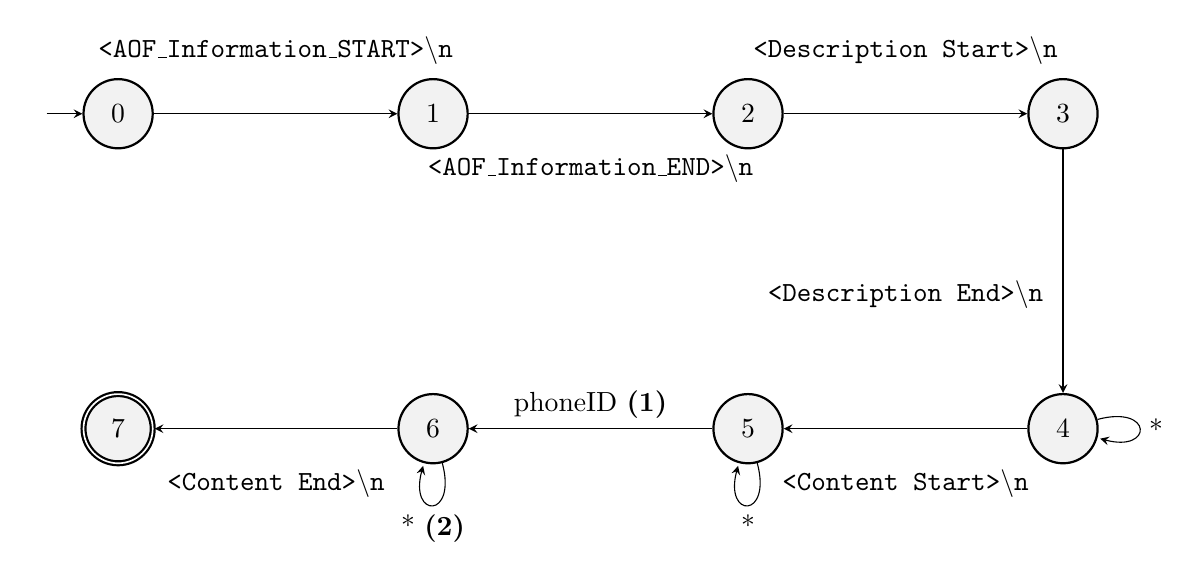
\begin{tikzpicture}
            \node[state, initial](s0) {0};
            \node[state, right of=s0](s1) {1};
            \node[state, right of=s1](s2) {2};
            \node[state, right of=s2](s3) {3};
            \node[state, below of=s3](s4) {4};
            \node[state, left of=s4](s5) {5};
            \node[state, left of=s5](s6) {6};
            \node[state, left of=s6, accepting](s7) {7};
            
            \draw (s0) edge[above] node[yshift=0.5cm]{\texttt{<AOF\_Information\_START>\textbackslash n}} (s1)
                (s1) edge[above] node[yshift=-1cm]{\texttt{<AOF\_Information\_END>\textbackslash n}} (s2)
                (s2) edge[above] node[yshift=0.5cm]{\texttt{<Description Start>\textbackslash n}} (s3)
                (s3) edge[below] node[xshift=-2cm]{\texttt{<Description End>\textbackslash n}} (s4)
                (s4) edge[above] node[yshift=-1cm]{\texttt{<Content Start>\textbackslash n}} (s5)
                (s4) edge[loop right] node{*} (s4)
                (s5) edge[loop below] node{*} (s5)
                (s5) edge[above] node{phoneID \textbf{(1)}} (s6)
                (s6) edge[above] node[yshift=-1cm]{\texttt{<Content End>\textbackslash n}} (s7)
                (s6) edge[loop below] node{* \textbf{(2)}} (s6)
                ;
        \end{tikzpicture}
        \caption{AOF input file analysis finite state machine. "*" character represents every possible symbol, bold numbers are action numbers.}
        \label{AOF input file analysis finite state machine}
    \end{figure}
    
    Finite state machine actions are:
    
    \begin{enumerate}[label=\textbf{(\arabic*)}: ]
        \item Get the phone ID, to use it in the name of the output file.
        \item If \texttt{QCLTE\_RRCMSG\_V2} found, write the message in the corresponding intermediate file ; if \texttt{QCLTE\_PSCELL} or \texttt{QCLTE\_PNCELL} found, populate EARFCN / PCI list from measurements taken ; if \texttt{QCLTE\_CELLINFO} found, set MCC and MNC values if they are not set.
    \end{enumerate}
    
    \subsubsection{Production of PCAP file}
    During this first step of file analysis, the PCAP file is produced using several tools. These tools are \texttt{text2pcap}, which write PCAP files using text file input, \texttt{mergecap}, which can merge several PCAP files into one, and \texttt{reordercap}, which can reorder chronologically packets in a PCAP file. \newline
    
    As we mentionned it, the PCAP file contains RRC messages. These message are dispatched on several logical channels (such as BCCH, PCCH...) and transport channels (BCH, DL-SCH...), used to distinguish types of messages \cite{bouguen_lte_2012}.
    Wireshark uses \textit{dissectors} to decode traces, which are parsers that decode network packet. For each channel, there is a dedicated dissector. The strategy is to produce temporary text files for each dissectors, which contains messages dates and traces in a text format in dedicated files, then to convert them into PCAP files using \texttt{text2pcap}.
    
    \begin{figure}[H]
        \centering
        \begin{lstlisting}[numbers=left, numberstyle=\ttfamily, breaklines=true]
2022-05-10 12:39:50.564365
0000 60 48 20 21 C0 FA 97 71 90 48 17 50 88 40 42 02 10 A0 88 84 6C C0

2022-05-10 12:39:50.564472
0000 00 02 59 3B 18 5F E5 42 D0 36 05 9A 80 D8 00 08 02 44 4E 31 D6 8A B0 7A 00 19 00 18 04 7B 31 A6 16 D0 61 60 08 03 10 00 00

2022-05-10 12:39:50.564594
0000 00 05 22 44 FF E2 6D 17 5E C4 A0\end{lstlisting}
        \caption{Extract from a file used by \texttt{text2pcap} generated from BCCH channel. Messages are dated and represented in hexadecimal notation}
        \label{BCCH text2pcap file}
    \end{figure}
    
    All of generated PCAP files are then merged into one PCAP file with \texttt{mergecap}, then this new PCAP file is reordered with \texttt{reordercap}.
    
    \subsubsection{AOF file data processing.}
    After the first step of parsing and producing of PCAP files, the AOF file is read a second time to extract data from \texttt{QCLTE\_PSCELL}, \texttt{QCLTE\_PNCELL} and \texttt{QCLTE\_CELLINFO}. This second read is done by the \texttt{XcalConverter.second\_read} function. \newline
    
    For this processing, data are structured in a Pandas DataFrame\footnote{\url{https://pandas.pydata.org/docs/reference/api/pandas.DataFrame.html}} like dictionary, which represents tabularly data. Given a set of fields \{\texttt{f1}, \texttt{f2}, \texttt{f3}, ...\} and rows (\texttt{v11}, \texttt{v12}, \texttt{v13}, ...) and ((\texttt{v21}, \texttt{v22}, \texttt{v23}, ...), the corresponding dictionary is:
    
    \begin{figure}[H]
        \centering
        \begin{lstlisting}[numbers=left, numberstyle=\ttfamily, breaklines=true, language=Python]
{
    f1: [v11, v21],
    f2: [v12, v22],
    f3: [v13, v23],
    ...
}\end{lstlisting}
        \caption{Python "DataFrame" dictionary.}
        \label{Python "DataFrame" dictionary}
    \end{figure}
    
        \begin{figure}[H]
        \centering
        \begin{lstlisting}[numbers=left, numberstyle=\ttfamily, breaklines=true, language=Python]
{
    f1: [v11, v21],
    f2: [v12, v22],
    f3: [v13, v23],
    ...
}\end{lstlisting}
        \caption{Python "DataFrame" dictionary.}
        \label{Python "DataFrame" dictionary}
    \end{figure}
    
    If we consider the example of \ref{Input file data organization.}, the structure is modified as shown in fig \ref{fig:PythonDataFramexAmple}.

    \begin{figure}[H]
        \centering
        \begin{lstlisting}[numbers=left, numberstyle=\ttfamily, breaklines=true, language=Python]
{
    "EARFCN1": [3000, 151, 151, 3000],
    "PCI1": [21, 21, 21, 21],
    ...
}\end{lstlisting}
        \caption{Example of Python "DataFrame" dictionary.}
        \label{fig:PythonDataFramexAmple}
    \end{figure}
    
 
    In this dictionary, the row \texttt{i} corresponds to the index \texttt{i} of lists associated to fields. The advantage of this data structure compared to Pandas Dataframe is it is more time efficient to modify. \newline
    
    Particularly, to store measurements by columns each dedicated to an EARFCN / PCI using this dictionary data structure, we use EARFCNs and PCIs found during the first reading of the file. Measurement from \texttt{QCLTE\_PSCELL} and \texttt{QCLTE\_PNCELL} are stored following this structure, each row being associated to a unique timestamp. In the case where several measurements with the same timestamp are found, values located in columns of the first measurement row are always kept, and values located in columns of the others measurement are copied in the first measurement row only if the corresponding column in the first measurement is empty. The name of corresponding entries in the output file is \texttt{MEASUREMENT}.\newline
    
    Concerning \texttt{QCLTE\_PSCELL} measurement values, they are also stored with the CINR in a \texttt{SERVING\_MEAS} entry, which corresponds to the serving cell. \texttt{QCLTE\_CELLINFO} data are stored in \texttt{CELLINFO} entries.
    
    \subsubsection{Estimation of geolocations}
    
    Measurements are geolocated in the AOF file with \texttt{GPS} traces. Since there is no \texttt{GPS} traces for each measurement, the location of measurement point is estimated by linear interpolation. \newline
    
    Let $\overrightarrow{G_1}, \overrightarrow{G_2} \in [-90, 90] \times [-180, 180]$ two vectors which represent two geolocations respectively taken at timestamps $t_1$ and $t_2$, $t_1 \leq t_2$ and $t_2, t_2 \in \mathbb{R}$, with:
    
    \begin{align}
        \overrightarrow{G_1} = \begin{pmatrix}
            x_1 \\ y_1
        \end{pmatrix} \ \text{and} \ \overrightarrow{G_2} = \begin{pmatrix}
            x_2 \\ y_2
        \end{pmatrix}
    \end{align}
    
    $x_1, x_2$ being latitudes and $y_1, y_2$ longitudes, and $M$ the sets of measurements taken between the two geolocations. Let $t: M \to \left[t_1, t_2\right]$ the function which associates every measurements of $M$ to their timestamp between $t_1$ and $t_2$. Geolocations of measurements in $M$ is estimated with the following function $\hat{G}$:
    
    \begin{align}
        \hat{G}\colon M & \longrightarrow \left[x_1, x_2\right] \times \left[y_1, y_2\right] \\[5pt]
        m & \longmapsto \begin{cases}
            \begin{pmatrix}
                \dfrac{t(m) - t_1}{t_2 - t_1} \times \left(x_b - x_a\right) + x_a\\[15pt]
                \dfrac{t(m) - t_1}{t_2 - t_1} \times \left(y_b - y_a\right) + y_a
            \end{pmatrix} \ \text{if} \ t_1 \neq t_2 \\[30pt]
            \overrightarrow{G_1} \ \text{otherwise}
        \end{cases}
    \end{align}
    
    It is possible that a series of measurement does not begins or does not terminates with a geolocation. In this case, we consider that $\overrightarrow{G_1} = \overrightarrow{G_2}$.
    
    \subsubsection{Content of the output file.}
    The output file contains the following fields:
    
    \begin{itemize}
        \item \texttt{MEAS\_EARFNCS}: list of all EARFCNs found, by ascending order. These EARFCNs are associated to PCIs in \texttt{MEAS\_EARFCNS} line. The \texttt{MEAS\_EARFCNS} line is used as a header line for the table of measurements.
        \item \texttt{MEAS\_PCIS}: list of all PCIs found, ordered by EARFCNs (\texttt{MEAS\_EARFNCS}). For a same EARFCN, corresponding PCIs are classed by ascending order.
        \item \texttt{CELLINFO}: contains information about a cell detected by the UE, such as EARFCN, PCI, TAC, CID and PLMN of this cell.
        \item \texttt{MEASURE\_SERVING}: contains information about the current serving cell (EARFCN, PCI) and measurement on Reference Signals (RSRP, RSSI, RSRQ, CINR).
        \item \texttt{MEASUREMENT}: stores measurements on reference signals of serving and neighbour cells, with each column associated to an EARFCN and PCI using \texttt{MEAS\_EARFCNS} and \texttt{MEAS\_PCIS}.
    \end{itemize}
    
    \subsection{Extraction of data from CSV Cartoradio files}
    This functionality of the software uses open data from Cartoradio, the ANFR website which reports radio antennas on French territory. These data are exportable in classic CSV format. The functionality produces several CSV file, one by operator, following the format used in previous parts, which contains informations about antennas of the operator which corresponds to the file and antennas sectors data. \newline
    
    Files taken in input are \texttt{Sites\_Cartoradio.csv} and \texttt{Antennes\_Emetteurs\_Bandes\_Cartoradio.csv}. These files contains the following data:
    
    \begin{itemize}
        \item \texttt{Sites\_Cartoradio.csv}: base station number, geolocation, postal address, city, support type...
        \item \texttt{Antennes\_Emetteurs\_Bandes\_Cartoradio.csv}: support and administrative numbers, antenna number, operator information, antenna type, directivity, technology (eg. LTE, GSM, UMTS...), frequency band...
    \end{itemize}
    
    \subsubsection{Cartoradio data processing}
    We will now designate in this part the file \texttt{Sites\_Cartoradio.csv} as the "site" file, and \\ \texttt{Antennes\_Emetteurs\_Bandes\_Cartoradio.csv} as the "antennas" file. The processing is done by the function \texttt{cartoradio.process\_cartoradio}.\newline
    
    The processing is based on the old program. \cite{trieu_visualization_2019}
    CSV datasets are first loaded in Pandas dataframes, using \texttt{pandas.read\_csv}. Antennas and sites datasets are joined over the support number, then, as it is required to create an output file for each operator, the dataset is grouped by operator (\texttt{Exploitant}), and only directive LTE antennas are kept. For each operator group, underground antennas (located in metros, for example) are rejected, and only antennas of base stations with a height superior or equals to 0 are kept. Antennas which doesn't meet this criteria will be stored by in a "rejected" file which corresponds to an operator (eg. \texttt{rejected\_SFR.csv}). Before writing the current antenna in an output file, the size of its sectors is calculated. Sector calculation is done following the number of antennas found on the base stations. \newline
    
     Let $i, j \in \mathbb{N}$, where $i$ identifies the current base station, and $j$ the current antenna. Let $\alpha_{i, j}$ the azimuth of the antenna $j$ of the base station $i$. In general, we have $\alpha_{i, j} < \alpha_{i, j +1}$. We designate as $L_i$ the number of antennas on a base station ; we have therefore $j \in \left[0, L_i - 1\right]$. Sectors are delimited with a minimum azimuth $\alpha^{\text{min}}_{i, j}$ and a maximum azimuth $\alpha^{\text{max}}_{i, j}$, expressed in degrees, and are calculated following these formulas \cite{trieu_visualization_2019}:
    
    \begin{align}
        \alpha^{\text{min}}_{i, j} = \begin{cases}
            \alpha_{i, j} - 60 & \text{if} \ L_i = 1 \\[10pt]
            \alpha^{\text{max}}_{i, j - 1} & \text{if} \ L_i > 1 \land j = L_i - 1 \\[10pt]
            \min\left(\dfrac{\alpha_{i, j} + \alpha_{i, L_i - 1} - 360}{2}, \dfrac{\alpha_{i, j} - \alpha_{i, j + 1}}{2}\right) & \text{if} \ L_i > 1 \land j = 0 \\[10pt]
            \min\left(\dfrac{\alpha_{i, j} + \alpha_{i, j - 1}}{2}, \dfrac{\alpha_{i, j} + \alpha_{i, j + 1}}{2}\right) & \text{if} \ L_i > 1 \land j > 0
        \end{cases}
    \end{align}
        
    \begin{align}
        \alpha^{\text{max}}_{i, j} = \begin{cases}
            \alpha_{i, j} + 60 & \text{if} \ L_i = 1 \\[10pt]
            \alpha^{\text{min}}_{i, 0} + 360 & \text{if} \ L_i > 1 \land j = L_i - 1 \\[10pt]
            \max\left(\dfrac{\alpha_{i, j} + \alpha_{i, L_i - 1} - 360}{2}, \dfrac{\alpha_{i, j} - \alpha_{i, j + 1}}{2}\right) & \text{if} \ L_i > 1 \land j = 0 \\[10pt]
            \max\left(\dfrac{\alpha_{i, j} + \alpha_{i, j - 1}}{2}, \dfrac{\alpha_{i, j} + \alpha_{i, j + 1}}{2}\right) & \text{if} \ L_i > 1 \land j > 0
        \end{cases}
    \end{align}
    
    Note that unidirectional antennas are supposed to have sector angle of 120°: this hypothesis is based on the fact antennas sectors has often an angle of approximately 120°. \newline
    
    From these calculations, delimiters lines are calculated: these lines are used by the visualization part. They are defined by the geographic coordinates of the base station $i$: $x^{\text{sta}}_{i} \in [-90, 90]$ (latitude) and $y^{\text{sta}}_{i}  \in [-180, 180]$ (longitude), and coordinates $x^{\text{del}}_{i, k} \in [-90, 90]$ and $y^{\text{del}}_{i, k} \in [-180, 180]$, based on each calculated azimuth limits $\alpha^{\text{lim}}_{i, k}$ of base station $i$, where $k \in \mathbb{N}$ is the $k$-th azimuth limit (note that an azimuth limit can be a minimum azimuth or a maximum azimuth of a sector):
    
    \begin{align}
        x^{\text{del}}_{i, k} = & x^{\text{sta}}_i + 0.3 \cos\left(\alpha^{\text{lim}}_{i, k} \times \dfrac{\pi}{180}\right) \\
        y^{\text{del}}_{i, k} = & y^{\text{sta}}_i + 0.3 \sin\left(\alpha^{\text{lim}}_{i, k} \times \dfrac{\pi}{180}\right)
    \end{align}
    
    Similarly, directivity lines of antennas are calculated for the visualization. For the antenna $j$ of the base station $i$, we calculate the latitude $x^{\text{dir}}_{i, j}$ and the longitude $y^{\text{dir}}_{i, j}$ of the extremity of the antenna directivity line as follows:
    
    \begin{align}
        x^{\text{\text{dir}}}_{i, j} = & x^{\text{sta}}_i + 0.0005 \cos\left(\alpha_{i, j} \times \dfrac{\pi}{180}\right) \\
        y^{\text{\text{dir}}}_{i, j} = & y^{\text{sta}}_i + 0.0005 \sin\left(\alpha_{i, j} \times \dfrac{\pi}{180}\right)
    \end{align}
    
    \subsubsection{Cartoradio processing output files}
    
    After these calculations done, antennas data are produced in CSV files which correspond to their operator. As said before, each operators have two CSV files: an output "sites" file, which contains data of kept antennas, and a "rejected" file which contains data of rejected antennas (underground antennas). These file contains the following entries:
    
    \begin{itemize}
        \item \texttt{BS\_ANTENNA}: contains antenna information, such as base station and antenna numbers, latitude and longitude of the base station, height, postal address, azimuth, directivity and sector information...
        \item \texttt{DELIMITER}: represents a delimiter which separates two sectors, contains data about antenna associated to the delimiter (base station and antenna numbers), latitude and longitude of the base station, and latitude and longitude of the extremity of the delimiter.
    \end{itemize}
    
    \subsection{Base station and measurements association process}
    
    The next functionality has for purpose to link measurements to a base station using EARFCN and PCI. During a measurement campaign on an urban-size area, we can considerate there is great chances that every EARFCN / PCI couple associated to measurements is unique, and we can use these couples to find to which base station a measurement point is related. \newline
    
    There is no trivial link between antennas and EARFCN / PCI, and it is necessary to calculate mathematical indicators. We will re-use criteria calculations used in the previous version of the program, and therefore base this part and the next formulas over \cite{trieu_visualization_2019}
    work: however, we will attempt reformulate more clearly and more exactly used calculations. \newline
    
    \subsubsection{Input data of the asscoiation process}
    
    First, this calculation takes two files as input: the file produced as output of the first step of AOF file data extraction (step 1 file), and the file produced as output of the second step of Cartoradio files data extraction (step 2 file) ; this calculation produces as output an association file. \newline
    
    The calculation is done with the class \texttt{association.CellAssociator}. The step 1 file is first read with the private function \texttt{CellAssociator.\_read\_measurements}. \texttt{CELLINFO} and \texttt{SERVING\_CELL} entries are stored in memory in DataFrame like structures, and \texttt{MEASUREMENTS} entries are directly written in the output file; \texttt{MEAS\_EARFCNS} and \texttt{MEAS\_PCIS} are also written in the output file, but are also used to create a list of EARFCN / PCI for further treatments. Then, the step 2 file is read with the private function \texttt{CellAssociator.\_read\_measurements}: data from \texttt{BS\_ANTENNA} entries are loaded into memory, and \texttt{DELIMITERS} entries are just copied in the output file.
    Data in memory are stored in two DataFrame, one which stores antennas and the other which stores associates \texttt{CELLINFO} data and serving cell measurements.\newline
    
    \subsubsection{Geometric calculation on cells}
    
    Using these data, we calculate first a theoretical estimation of the cells, using Voronoi diagrams, from the positions of the sites. This calculation, using here the class \texttt{scipy.spatial.Voronoi} from the SciPy library, creates geometrical cells around each site. The cell of a site corresponds to the set of point which are nearest of this base station than other base stations.
    
    \begin{figure}[H]
        \centering
        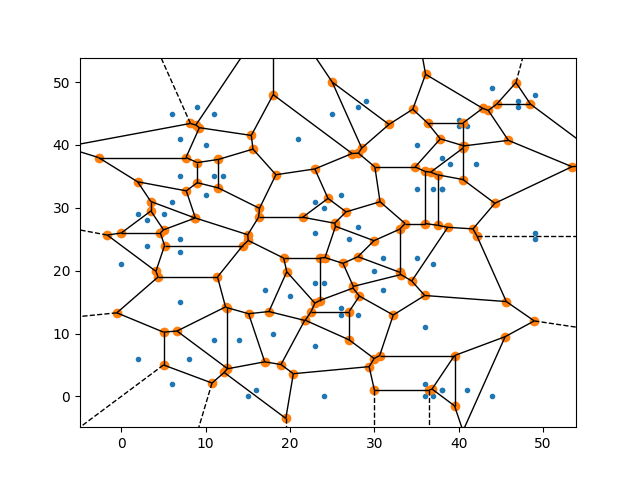
\includegraphics[width=0.75\textwidth]{vor_scipy.png}
        \caption{Voronoi diagram of a set of 75 points on $\llbracket0, 49\rrbracket^2$ randomly generated with \texttt{random.randrange}, using SciPy's \texttt{Voronoi} class, \texttt{scipy.spatial.voronoi\_plot\_2d}, and \texttt{matplotlib.pyplot}.}
        \label{Voronoi Cells}
    \end{figure}
    
    After the initial cell calculations, it is required to remove "open" cells: these cells are situated at the extremities of the set of points, and extend in infinite directions. In SciPy, input points (base station points here) are stored in the array \texttt{Voronoi.points}. For each point of index \texttt{i}, corresponding region number is stored in the array \texttt{Voronoi.point\_region}, at the index \texttt{i}. Then, we can finally get the corresponding region with \texttt{Voronoi.regions} array, each element of this array being a list of indexes of elements from \texttt{Voronoi.vertices} \cite{the_scipy_community_scipyspatialvoronoi_nodate}.
    In the case of the current cell is an open cell, at least one vertex will be represented by the index \texttt{-1} under default parameters. \cite{the_scipy_community_scipyspatialvoronoi_nodate}.
    We can eliminate these cells, as the calculation requires cells are convex polygons. Results of this calculation are stored in a DataFrame-like dictionary containing latitude, longitude of each site and the corresponding region number. \newline
    
    \begin{figure}[H]
        \centering
        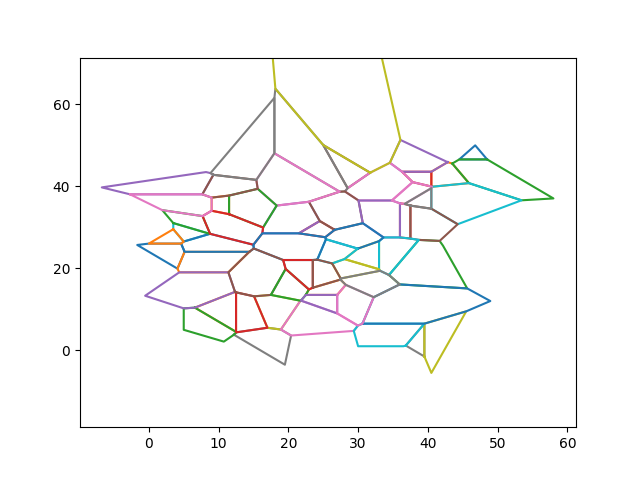
\includegraphics[width=0.75\textwidth]{vor_filtered.png}
        \caption{Voronoi diagram of the same set of points than the last figure, after removing open cells, represented using \texttt{shapely} and \texttt{matplotlib.pyplot}.}
        \label{Voronoi Cells}
    \end{figure}
    
    We merge then antennas and Voronoi DataFrame issued from Voronoi dictionary over the latitude and longitude, to associate to each antenna the corresponding Voronoi cell. Following \cite{trieu_visualization_2019}
    notations, we will now name $\mathcal{V}_i$ the Voronoi cell of the base station $i$. \newline
    
    Then, for each group of serving cell measured points of the point association DataFrame with the same EARFCN / PCI, we will calculate the convex hull of these points, using the Shapely library and its class \texttt{shapely.MultiPoint}, and the property \texttt{convex\_hull} of this class. Mathematically, the convex hull of set of points is the smallest convex polygon that contains these points, i.e. the smallest possible polygon which contains all point of the set, and where for two arbitrary points inside the polygon, the line between the two points is also in the polygon. Also according \cite{trieu_visualization_2019}
    notation, for a group of points of same EARFCN / PCI that we will note now $\mathcal{S}_n$, $n \in \mathbb{N}$, we will now use $\mathcal{C}_n$ to designate the corresponding convex hull of this group. \newline
    
    \begin{figure}[H]
        \centering
        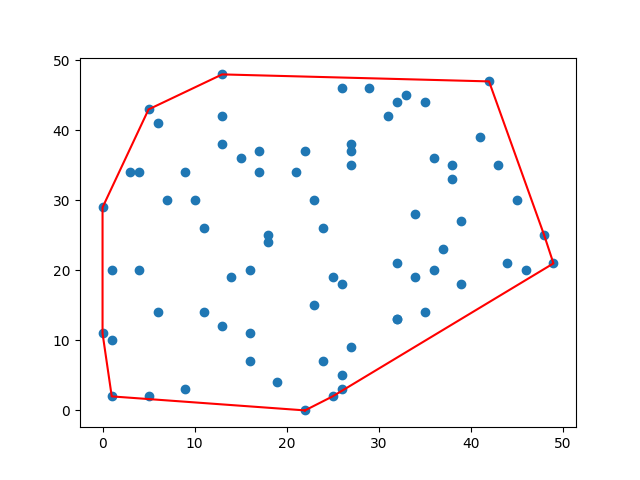
\includegraphics[width=0.75\textwidth]{convex_hull.png}
        \caption{Set of 75 points on $\llbracket0, 49\rrbracket^2$ randomly generated with \texttt{random.randrange} and its convex hull in red, using \texttt{convex\_hull} property of \texttt{shapely.geometry.MultiPoint}, plotted with \texttt{matplotlib.pyplot}.}
        \label{Voronoi Cells}
    \end{figure}
    
    \subsubsection{Use of vectorized function for the calculation}
    
    For the following part, we will first introduce the concept of vectorized functions, massively used in this part through the usage of the NumPy library. \newline
    
    Let $f: E \to F$ an arbitrary function mapping elements from $E$ to $F$. Note there is no particular constraint on the function unless we can considerate $f$ as a total function in the case of the Python programming language, as a function with without return value will return always \texttt{None}. Ordinarly, to calculate the value of $F$ associated to $e \in E$ with $f$, we need just to calculate $f(e)$. That implies if we want to calculate a sequence $v: \llbracket0, L\rrbracket \to F$, $L \in \mathbb{N}$ of numbers associated to the corresponding sequence $u: \llbracket0, L\rrbracket \to E$ of numbers from $E$, we need to iterate over the sequence $u$ following $k \in \llbracket0, L\rrbracket$ to calculate $v_k = f\left(u_k\right)$ using for example in an imperative programming language a \texttt{for} loop, which can be really redundant in program. \newline
    
    A solution to this is the use of vectorized functions. Instead of iterating over sequence of numbers from $E$ to calculate the corresponding sequence of numbers of $F$, taking the example of $u$ and $v$, we can use vectors $\overrightarrow{u'}$ and $\overrightarrow{v'}$, with:
    
    \begin{align}
        \overrightarrow{u'} = \begin{bmatrix}
            u_0 \\
            u_1 \\
            u_2 \\
            \vdots \\
            u_L
        \end{bmatrix} \ \text{and} \ \overrightarrow{v'} = \begin{bmatrix}
            v_0 \\
            v_1 \\
            v_2 \\
            \vdots \\
            v_L
        \end{bmatrix}
    \end{align}
    
    A vectorized function follows this principle: instead of mapping an element of a arbitrary set $E$ to another element of another set of $F$ using a function $f$, it is possible to map a series of $n \in \mathbb{N}$ elements from $E$ represented with a vector from $E^n$ to a vector from $F^n$, representing the associated series of number from $F$, using the vectorized version $f_\text{V}$ of the function $f$, with the following definition, with $e_k \in E$ and $f_k \in K$, $k \in \llbracket0, n\rrbracket$:
    
    \begin{align}
        f_\text{V}: E^n & \longrightarrow  F^n \\[5pt]
        \begin{bmatrix}
            e_0 \\
            e_1 \\
            e_2 \\
            \vdots \\
            e_n
        \end{bmatrix} & \longmapsto  \begin{bmatrix}
            f(e_0) \\
            f(e_1) \\
            f(e_2) \\
            \vdots \\
            f(e_n)
        \end{bmatrix}
    \end{align}
    
    Using NumPy, it is possible to use as vector lists or NumPy arrays. A lot of standard mathematical functions have a vectorized version in NumPy (\texttt{numpy.cos}, \texttt{numpy.abs}...), and it is possible to create the vectorized version of an arbitrary function using \texttt{numpy.vectorize}. \newline
    
    The reason to use these vectorized functions its they allow to calculate values over arrays of number concisely. We will find this situation in the following calculations.
    
    \subsubsection{Cell association calculation}
    
    In ordrer to associate each measurement to an antenna, \cite{trieu_visualization_2019}
    uses several criteria. These criteria are based on the angle between the north axis and the line between the point and the corresponding site, and on the belonging of the point to a cell. \newline
    
    To do properly angular-based calculation, latitude and longitude, expressed in degrees, which are spheric coordinates, are projected over a plane: calculation used in \cite{trieu_visualization_2019}
    to do so are the following: let $A_i = \left(\phi_i, \lambda_i\right)$ geolocation of the $i$-th site, and $X_k = \left(\phi_k, \lambda_k\right)$ geolocation of a measurement, with $i, k \in \mathbb{N}$. We calculate relative coordinates $\left(d_{\text{N}, i, k}, d_{\text{E}, i, k}\right)$ over plane projection of the point $X_k$, following the site $A_i$. These relative coordinates are calculated in the old program, based on \cite{trieu_visualization_2019}
    as the following:
    
    \begin{align}
        d_{\text{N}, i, k} & = \dfrac{\pi}{180}\left(\phi_k - \phi_i\right) \\
        d_{\text{E}, i, k} & = \dfrac{\pi}{180}\left(\lambda_k - \lambda_i\right) \cos(\phi_i)
    \end{align}
    
    \texttt{numpy.array} containing latitudes and longitudes are used for this calculus, as they uses vectorized mathematical operators overloads; \texttt{numpy.cos} function is also used. \newline
    
    From these coordinates, we calculate the angle $\alpha\left(A_i, X_k\right)$, which is given by the following formula, defined in \cite{trieu_visualization_2019}
  :
    
    \begin{align}
        \alpha\left(A_i, X_k\right) = \arctan2\left(d_{\text{E}, i, k}, d_{\text{N}, i, k}\right)
    \end{align}
    
    \texttt{numpy.arctan2} vectorized function is used here.
    
    \begin{figure}[H]
	\centering
	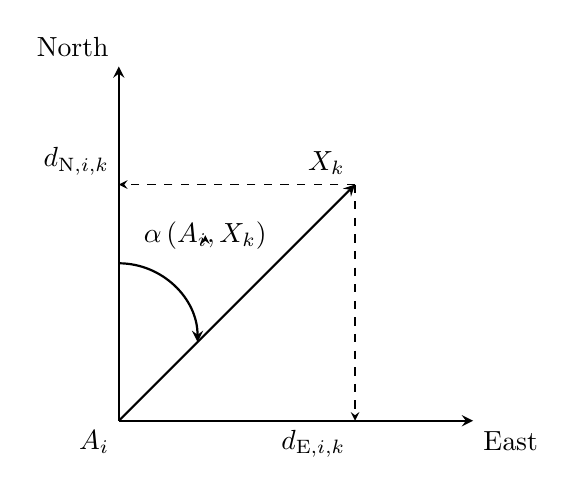
\begin{tikzpicture}
	\draw[thick,->] (0,0) -- (0,4.5) node[anchor=south east] {North};
	\draw[thick,->] (0,0) -- (4.5,0) node[anchor=north west] {East};
	\draw[thick,->] (0,0) -- (3,3) node[anchor=south east] {$X_k$};
	\draw[dashed] (3,3) -- (3,0) node[anchor=north east] {$d_{\text{E}, i, k}$};
	\draw[dashed] (3,3) -- (0,3) node[anchor=south east] {$d_{\text{N}, i, k}$};
	\path (0,0) node [anchor=north east] {$A_i$};
	\draw[thick,<-]  (1,1) arc (0:90:1cm);
	\draw(65:2.6cm) node {$\alpha\left(A_i,X_k\right)$};	
	\end{tikzpicture}
	\caption{Relative coordinates of $X_k$ from $A_i$ and angle $\alpha\left(A_i, X_k\right)$. Figure by Hoang TRIEU, extracted from \cite{trieu_visualization_2019}.}
	\label{Plane coords and angle}
\end{figure}

    Then, it is possible to calculate association criteria. First, we attribute to each point of indice $k \in \mathbb{N}$ in a group $\mathcal{S}_n$, $n \in \mathbb{N}$ with a RSRP $R_k$ a weight which is given by the following formula \cite{trieu_visualization_2019}:
    
    \begin{align}
        w_k = \begin{cases}
        0.15  & \text {if }  R_k \leq -100 \text { dBm}\\
        0.6  &\text {if }  -100 \text { dBm} < R_k < -80 \text { dBm} \\
        1  &\text {if }  R_k \geq  -80 \text { dBm}
        \end{cases}
    \end{align}
    
    Weight function is vectorized in the python program using \texttt{numpy.vectorize}.
    
    Based on these weights, we calculate now for the group $\mathcal{C}_n$ the angular criteria $\sigma_{i, j, n}$ for each antenna of indice $j \in \mathbb{N}$ from the site of indice $i \in \mathbb{N}$ \cite{trieu_visualization_2019}:
    
    \begin{align}
        \sigma_{i, j, n} = \begin{cases}
            0 & \text{if} \ \mathcal{V}_i \cap \mathcal{C}_n = \varnothing \\[10pt]
            \displaystyle \sum_{k=1}^{\left|\mathcal{C}_n\right|}{w_k\dfrac{\left[\alpha^\text{min}_{i, j} < x < \alpha^\text{max}_{i, j}\right]\left(\alpha\left(A_i,X_k\right)\right)}{\left|S_k\right|}} & \text{otherwise}
        \end{cases}
    \end{align}
    
    This indicator is calculated using a function vectorized with \texttt{numpy.vectorize}.
    
    Note that we use the notation $\left[\alpha^\text{min}_{i, j} < x < \alpha^\text{max}_{i, j}\right]\left(\alpha\left(A_i,X_k\right)\right)$. This notation is know as Iverson bracket. Let $P$ be a first-order logic predicate over a domain $E$. We define the Iverson bracket $[P]$ as follows ($\neg$ means not):
    
    \begin{align}
        [P]: E & \longrightarrow  \{0, 1\} \\[5pt]
        x & \longmapsto  \begin{cases}
            0 & \text{if} \ \neg P(x) \\
            1 & \text{if} \ P(x)
        \end{cases}
    \end{align}
    
    This mean that if we pass as argument of $[P]$ a value $x$, if $x$ follows the condition defined by $P$, the function will return 1, if not it will return 0. Here, we use as condition that the angle $\alpha\left(A_i,X_k\right)$ must be included between the minimum and maximum sector of the antenna $j$ of the site $i$. This criteria consists of the average of the belonging value of points of $\mathcal{C}_k$ to the sector of a given antenna.
    \newpage
    
    The second criteria is the cell belonging criteria of the points of $\mathcal{C}_n$ to the cell $\mathcal{V}_i$, with taking account of the belonging of the point to the sector of the antenna $j$. This indicator is noted $\psi_{i, j, n}$ \cite{trieu_visualization_2019}: 
    
    \begin{align}
        \psi_{i, j, n} = \begin{cases}
            0 & \text{if} \ \mathcal{V}_i \cap \mathcal{C}_n = \varnothing \\[10pt]
            \displaystyle \sum_{k=1}^{\left|\mathcal{C}_n\right|}{w_k\dfrac{\mathbbm{1}_{\mathcal{V}_i}\left(X_k\right) \times \left[\alpha^\text{min}_{i, j} < x < \alpha^\text{max}_{i, j}\right]\left(\alpha\left(A_i,X_k\right)\right)}{\left|S_k\right|}} & \text{otherwise}
        \end{cases}
    \end{align}
    
    The notation $\mathbbm{1}_{\mathcal{V}_i}$ corresponds to an indicator function, which is a particular case of Iverson brackets defined as follows: $\mathbbm{1}_A = [x \in A]$, $A$ being an arbitrary set. In other words, the function will return 1 if a given argument $x$ belongs to $A$, 0 if not. Here, we want to check if the point belongs to the Voronoi cell of the antenna. \newline
    
    The indicator is calculated following using by multiplying the result vector of calculations of $\mathbbm{1}_{\mathcal{V}_i}\left(X_k\right)$ by the result vector of calculations of $w_k \times \left[\alpha^\text{min}_{i, j} < x < \alpha^\text{max}_{i, j}\right]\left(\alpha\left(A_i,X_k\right)\right)$, kept from the calculation of the first criteria, then calculate the average of the obtained vector. \newline
    
    With $\sigma_{i, j, n}$ and $\psi_{i, j, n}$ being calculated, these indicators need to be merged into a final indicator, called $\theta_{i, j, n}$, defined as follows \cite{trieu_visualization_2019}:
    
    \begin{align}
        \theta_{i, j, n} = \begin{cases}
        0  & \text {if }\psi_{i,j,n}<0.25 \\
        0.2 \psi_{i,j,n} + 0.8 \sigma_{i,j,n} & \text{ otherwise.}
        \end{cases}
    \end{align}
    
    The calculation of $\theta_{i, j, n}$ is not vectorized, as its calculation is based on only two values, $\sigma_{i, j, n}$ and $\psi_{i, j, n}$, and therefore does not need to be calculated from a large series of values. \newline
    
    The presence of the threshold value 0.25 allows to exclude group of points very partially included in a sector, which can be considered as not significant for the association \cite{trieu_visualization_2019}. \newline
    
    $\theta$ criteria is calculated for all antennas $j$ from all cells $i$, for each group $n$. Then, we pose the value $\theta_{i_\text{max}, j_\text{max}, n}$ as the maximum $\theta$ value associated to the group of point $S_n$. Association of $S_n$ to the antenna $j$ of the site $i$ will be done only if \cite{trieu_visualization_2019}:
    
    \begin{align}
        \forall i', j', \left(i_\text{max} \neq i' \land j_\text{max} \neq j' \land \dfrac{\theta_{i', j', n}}{\theta_{i_\text{max}, j_\text{max}, n}} \neq 0 \land \theta_{i_\text{max}, j_\text{max}, n} \neq 0 \right) \\[10px]
        \Longrightarrow \left|\log\left(\dfrac{\theta_{i', j', n}}{\theta_{i_\text{max}, j_\text{max}, n}}\right)\right| > 0.08
    \end{align}
    
    i. e. for all $i'$ and $j'$, the condition in (22) is false or the condition at the left of the arrow in (23) is true. \newline
    
    Using this condition, several antennas can be associated to a same group, as surface in the angle of the sector of an antenna extents infinitely. The last step of the treatment consists to choose the group $\mathcal{S}_n$ associated to the convex polygon $\mathcal{C}_n$ such as the distance between the associate antenna and the nearest point of $\mathcal{C}_n$ is minimal \cite{trieu_visualization_2019}. This calculation is done using Shapely library, by calculating a projection number on the polygon, which can be used to interpolate the corresponding point over the polygon.
    
    \subsubsection{Warning}
    
    There can be several groups of measurement point for the same sector. Only one should be kept but this is not implemented. 
    
    \subsubsection{Content of the association output file}
    
    The output file\footnote{If the imput file is xxx then the output file is \texttt{assoc\_xxx}} contains the following fields:
    
    \begin{itemize}
        \item \texttt{MEAS\_EARFCNS}: list of all EARFCNs in (EARFCN, PCI) pairs found during the measurement campaign.
        \item \texttt{MEAS\_PCIS}: list of all PCIs in (EARFCN, PCI) pairs found during the measurement campaign.
        \item \texttt{MEASUREMENT}: global measurements associated to (EARFCN, PCI) pairs following columns. Can be RSRP, RSRQ or RSSI measurements.
        \item \texttt{DELIMITER}: used to draw antennas sectors delimitation lines.
        \item \texttt{BS\_ANT\_DIR}: used to draw antennas directivity lines.
        \item \texttt{ASSOC}: defines an association between a Cartoradio number (base station), an antenna number and TAC, CID, EARFCN, PCI values.
        \item \texttt{POINT}: defines a point with its latitude and longitude, its TAC, CID, EARFCN and PCI values and its measurements (RSRP, RSRQ, RSSI, CINR).
    \end{itemize}
    
    \newpage
    
    \section{Visualization}

    This part aims to document the web front-end application used to visualize measurement campaigns.
    We will first focus on the general structure of this part, before presenting briefly the some of the inner
    workings of this application.
    
    \subsection{JavaScript application structure}

    This application, stored in the folder \texttt{web\_ui}, is splitted into several files, which are
    themselves stored in several folders.

    In the main folder, the application web page is stored in \texttt{index.html}. This file a HyperText Markup
    Language File (HTML), and contains the layout of the application. Several styles are applied on this web page, user
    defined styles being stored in the \texttt{styles} folder, in the file \texttt{frontstyle.css}, which is
    a Cascading Style Sheet (CSS) file. \newline

    However, the main application uses a JavaScript program stored in the folder \texttt{scripts}, which contains
    the following JavaScript files:

    \begin{itemize}
        \item \texttt{app.js}: main app file. It contains the class \texttt{app.App}, which wraps the global state
        of the application, such as the map or selected data, defines events handlers that allows the user
        to interact with the application, and updates the user interface when necessary.
        \item \texttt{csvread.js}: this file contains the class \texttt{csvread.CSVReader}, which is used to read the
        CSV file passed as an input of the application. Data from the file are also stored in this class.
        \item \texttt{drawing.js}: this file contains the class \texttt{drawing.Map}, which can wrap the map component
        of the user interface, and is used to draw layers on the map, following the user selection, with dedicated methods.
        \item \texttt{processing.js}: processes antennas, cells and sectors data into drawable geographical information.
        \item \texttt{styles.js}: this file defines function to style components of the map (points, cells, heatmap...).
        \item \texttt{utils.js}: this file contains functions for various utilities, which are not classable in the other
        files (array manipulation, object copy...).
    \end{itemize}

    The program also use several libraries, stored in the the \texttt{library} folder\footnote{Note there in this folder several legacy unused libraries.} 
    which are the following:

    \begin{itemize}
        \item Bootstrap: used to define the layout of the user interface.
        \item Leaflet: defines the map component \texttt{L.Map} used in the UI.
        \item d3: \textit{Data Driven Documents}, used as a dependency to visualize data.
        \item Leaflet-d3: extension to Leaflet and d3 to visualize data, used for heatmaps.
        \item turf.js: used to do calculations over the GeoJSON format\footnote{Format of JavaScript objects
        standardized by the RFC-7946 (\url{https://www.rfc-editor.org/rfc/rfc7946.txt})}
    \end{itemize}

    \subsection{Aspects of the inner working of the application}

    \subsubsection{Selection of EARFCNs and PCIs}
    One of the most important features of the application is the selection by the use of EARFCNs and PCIs
    of data to be displayed. This selection is mostly managed by the \texttt{utils.subEarpcis} function,
    but is also managed by other functions. Usually, these functions take two parameters, \texttt{earfcns} and
    \texttt{pcis}, which have as default values the value \texttt{null}. An \texttt{earfcns} parameter which
    is \texttt{null} means that every EARFCN need to be selected,  a \texttt{pcis} parameter which
    is \texttt{null} means that every PCI need to be selected, and two \texttt{null} parameters means that every
    EARFCN / PCI must be selected. To select no EARFCN / PCI pair, the two parameters must be empty arrays (\texttt{[]}).
    To select existing EARFCNs and PCIs, the \texttt{earfcns} parameter must contains EARFCNs of chosen pairs, and
    \texttt{pcis} parameter must contain corresponding PCIs.

    \subsubsection{Management of layers}

    Following selected EARFCNs and PCIs, layers of data to display on the map must be managed. 
    The only option to hide a layer using Leaflet is to remove it from the map; that implies layers
    must be stored in memory, and must be identifiables.\newline

    Measurement layers, using hexagonal-tiled heatmaps, are modified by removing their points of data, and
    filtering then re-adding them following selected EARFCNs and PCIs. These data points are stored in arrays
    and contains a longitude, a latitude and value. Serving measurements layers and global measurement
    layers are displayed separately, following if a the user selected serving measurements or not. \newline
    
    Point layers (TAC and PCI) consist in fact in groups of layers. These layers are stored in dictionary-like objects, each associated
    to an EARFCN and PCI, and are added or removed from the following the user selection. \newline

    Antennas and theoretical cell layers are managed more easily, as they are GeoJSON object created with
    turf.js: in particular, the cell layer contains the Voronoi diagram of theoretical cells, generated by
    turf.js from antenna datas. \newline

    Associated site layer consists in a group of tooltips markers, generated from antennas and association data,
    and bound to a tooltipn which contains checkboxes for the selection of EARFCNs and PCIs by sites. These checkboxes
    are added from the current user selection through EARFCN and PCI selection drop down menus, and are automatically
    checked or not following the previous checkbox selection before the drawing of the mark.

    \subsubsection{Automatic generation of the color gradient for heatmaps}

    Heatmap gradient use cold colors for low values, "intermediate" colors for intermediate values, and hot
    colors for high values. This gradient is calculated by Leaflet-d3, using a list of given color values. \newline

    This list can be generated automatically, using the HSL (Hue-Saturation-Lightness) color system. This color system
    defines each color over three values $(h, s, l) \in [0, 360] \times [0, 1] \times [0, 1]$. We can generate the required
    colors by decreasing $h$ value over $[0, 240]$, with $s = 1$ to have fully saturated color and $l = 0.5$ to
    not have too "white" or too "black" colors. Following this principle, to generate a set of $n$, color, we can decrease
    $h$ by $\dfrac{240}{n}$ steps. We can use to do easily this the d3 library, with \texttt{d3.hsl} function, and use on the
    return value of this function the function \texttt{formatHex()} to obtain the hexadimal RGB value of the color.

    \begin{figure}
        \centering
        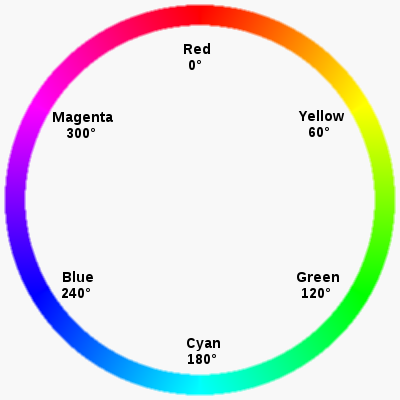
\includegraphics[width=0.5\textwidth]{RGB_color_circle.png}
        \caption{HSL color circle. Used color are situated between 0° and 240°, with cold colors situated around 240° and hot colors around 0°. \newline By Steve11235 - Own work, CC0, \url{https://commons.wikimedia.org/w/index.php?curid=20576730}}
        \label{Colors HSL}
    \end{figure}

    \subsubsection{Updating policy of the UI}
    As the user can frequently filter data on the visualization, several functions are defined in order to update the user interface.
    They are all situated in the file \texttt{app.js}:

    \begin{itemize}
        \item \texttt{app.update}: updates layers using selected EARFCN and PCIs by redrawing them. Called on
        every change of selected EARFCN and / or PCI, from selectors or checkboxes.
        \item \texttt{app.updateDisplay}: only hide or show layer, doesn't update its data.
        Called every time a layer is shown or hide (when using the checkboxes at the right of the UI for example).
        \item \texttt{app.updateAssocs}: updates the associations marks, and the checkboxes in their popups. Called every time EARFCN / PCI data are changed.
    \end{itemize}
    
    \section{Conclusion}
    This program have been built on a previous program, which had calculations and data processings on which the current program have been built. If the current program succeeds to use data of Xcal-M file to provide more detailled visualisation, allowing the user to choose more easily on which EARFCN, PCI and base station it wants to visualize measurements, an huge adaption work has however been done, to enhance the program maintainability and allow the integration of new functionalities. The reimplementation of functionalities, such as association between cells and measurements, increased calculation speeds, but have also proven some limits, as the association can incorrectly asscociate several PCIs to a same antenna. Some of the old vizualisation features, such as the estimating of the coverage of an antenna using convex polygons, have not been reimplemented. The improvement, and the integration of additional functionalities, could be the base of further works on this project.
    
    \addcontentsline{toc}{section}{Bibliography}
    \printbibliography
    
\end{document}